\documentclass{article}
\usepackage[margin=20mm]{geometry}
\usepackage{graphicx}
\usepackage{booktabs}
\begin{document}
\title{Additional TensorFVM analytic benchmarks}\maketitle
\section{Problems and methods}
ABC: $\mathbf u=(\sin z+\cos y,\sin x+\cos z,\sin y+\cos x)e^{-\nu t}$; $p=-\rho|\mathbf u|^2/2+C$. Shear: $u=\sin(y-0.7t)e^{-\nu t}$, $v=0.7$, $w=0$, $p=0$. Production MAC midpoint, full symmetric stress, shared conservative flux, compatible FFT projection. Velocity at final face coordinates; pressure at last midpoint cell coordinates. Strict physical error below 3 percent.
\section{Results}
\begin{tabular}{lllrr}\toprule Case & Grid & Role & Velocity error (percent) & Pass\\\midrule
abc & 24x24x24 & spatial & 0.005699 & True \\
abc & 32x32x32 & spatial & 0.003209 & True \\
abc & 48x48x48 & spatial & 0.001427 & True \\
advected-shear & 16x16x4 & spatial & 0.620363 & True \\
advected-shear & 24x24x4 & spatial & 0.276903 & True \\
advected-shear & 32x32x4 & spatial & 0.156024 & True \\
abc & 16x16x16 & negative-control & 0.012786 & False \\
advected-shear-lbm & 32x32 & comparison & 0.230176 & True \\
advected-shear-lbm & 64x64 & comparison & 0.054381 & True \\
\bottomrule\end{tabular}
\section{Discussion}
The n16 ABC pressure control fails and is preserved. Shear pressure error uses initial dynamic pressure scaling because its exact value is zero. D2Q9 is only compared with two-dimensional shear. Raw states, independent audit and source hashes are included. No cylinder, free-surface or icebreaking qualification is asserted.
\subsection{abc 32x32x32}
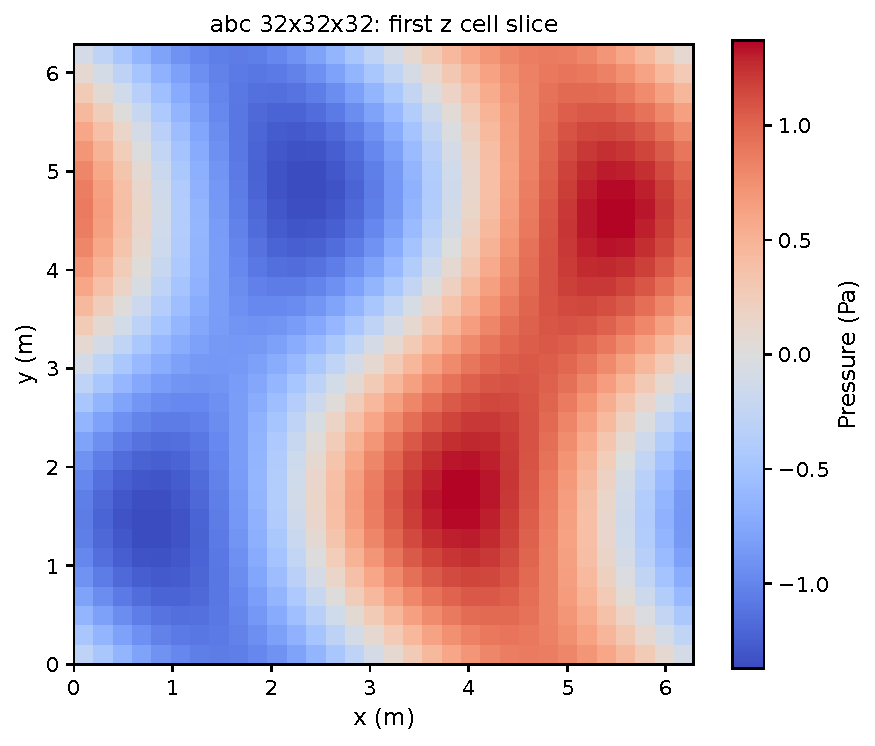
\includegraphics[width=0.48\linewidth]{abc-32/figures/pressure.pdf}
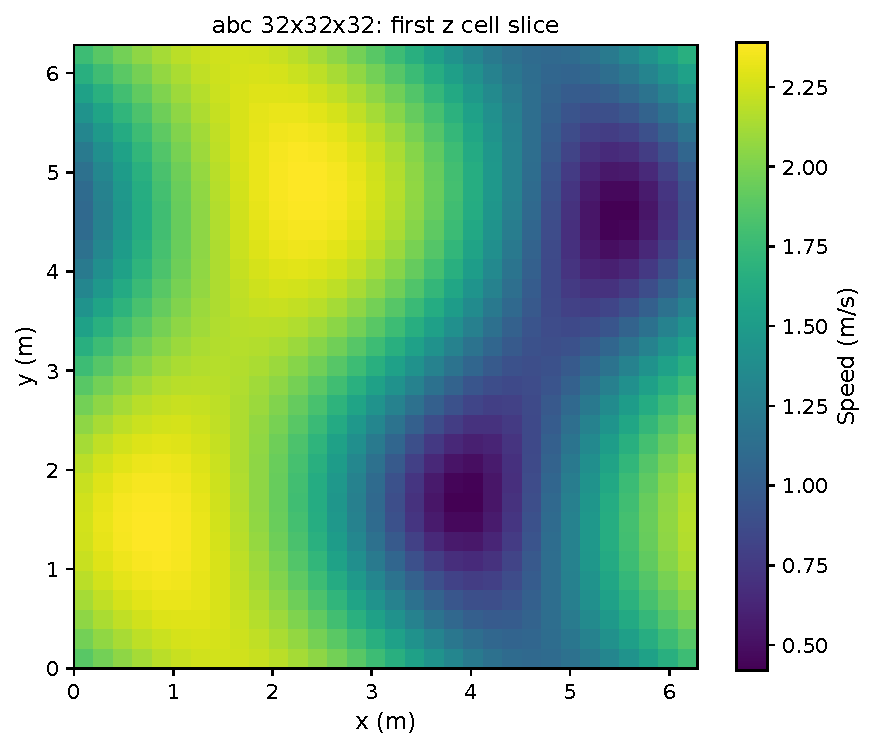
\includegraphics[width=0.48\linewidth]{abc-32/figures/speed.pdf}
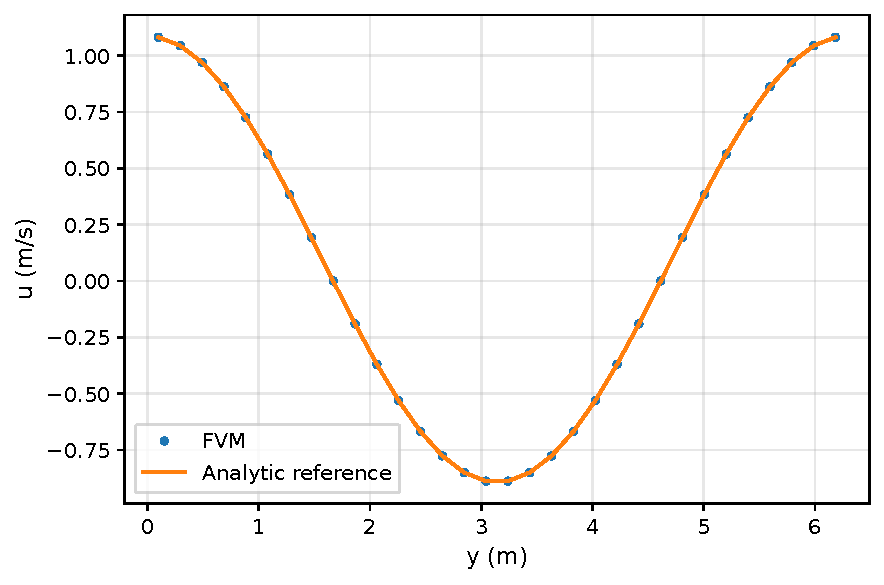
\includegraphics[width=0.48\linewidth]{abc-32/figures/velocity-profile.pdf}
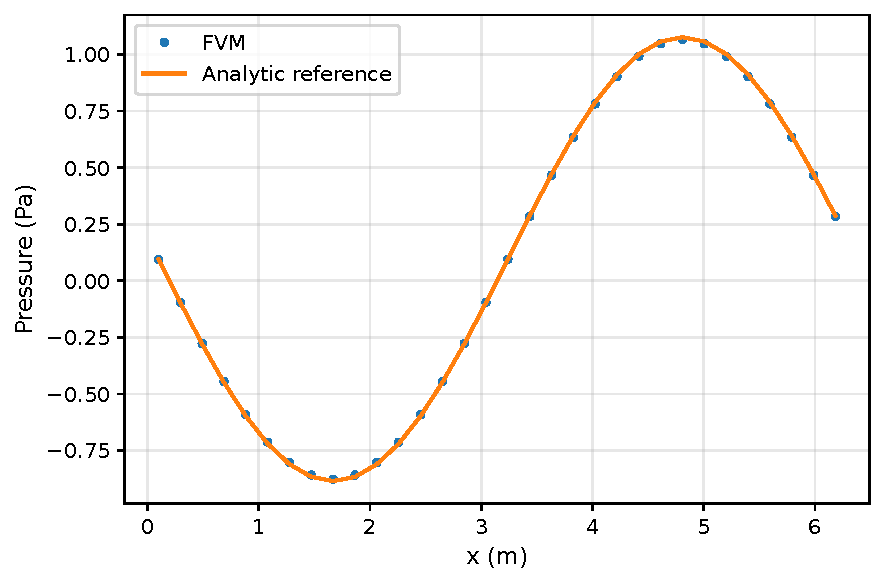
\includegraphics[width=0.48\linewidth]{abc-32/figures/pressure-curve.pdf}
\subsection{abc 48x48x48}
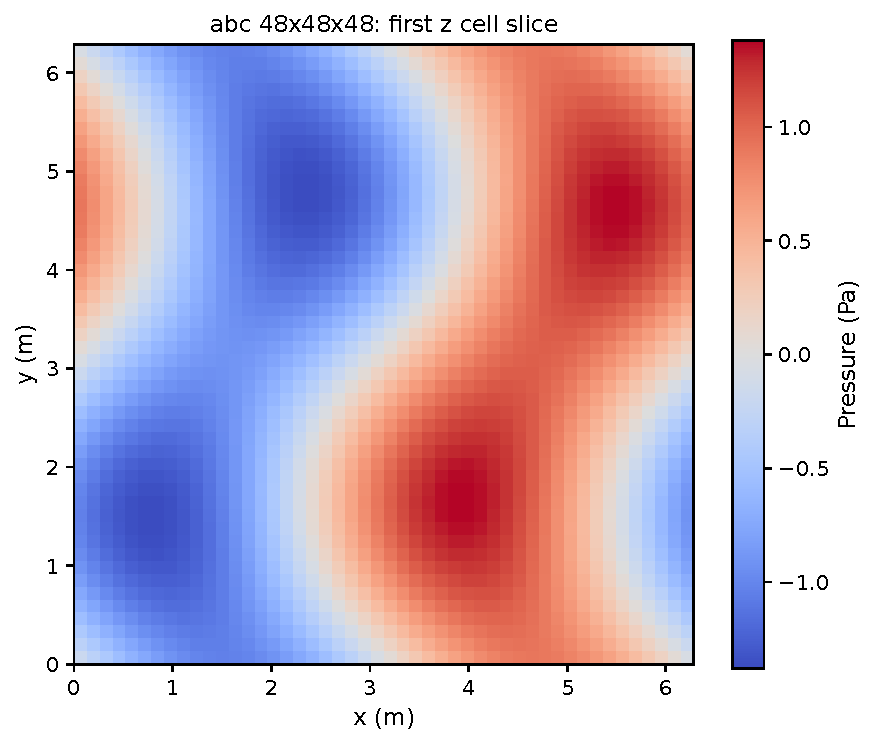
\includegraphics[width=0.48\linewidth]{abc-48/figures/pressure.pdf}
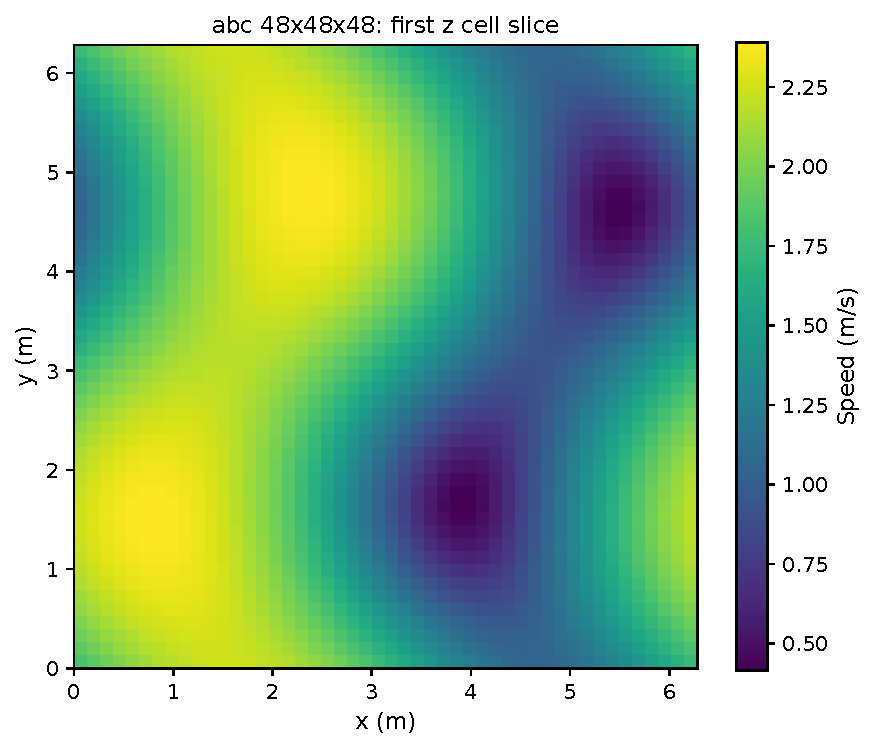
\includegraphics[width=0.48\linewidth]{abc-48/figures/speed.pdf}
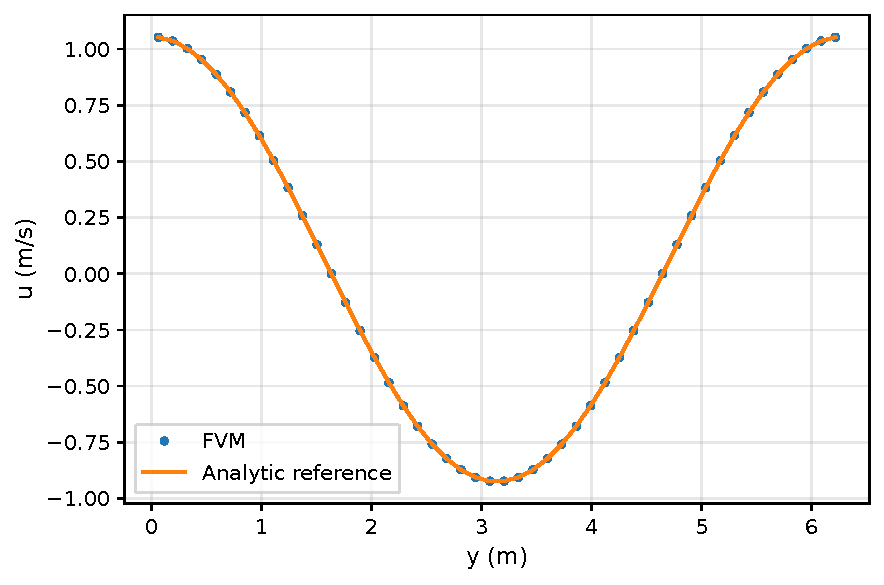
\includegraphics[width=0.48\linewidth]{abc-48/figures/velocity-profile.pdf}
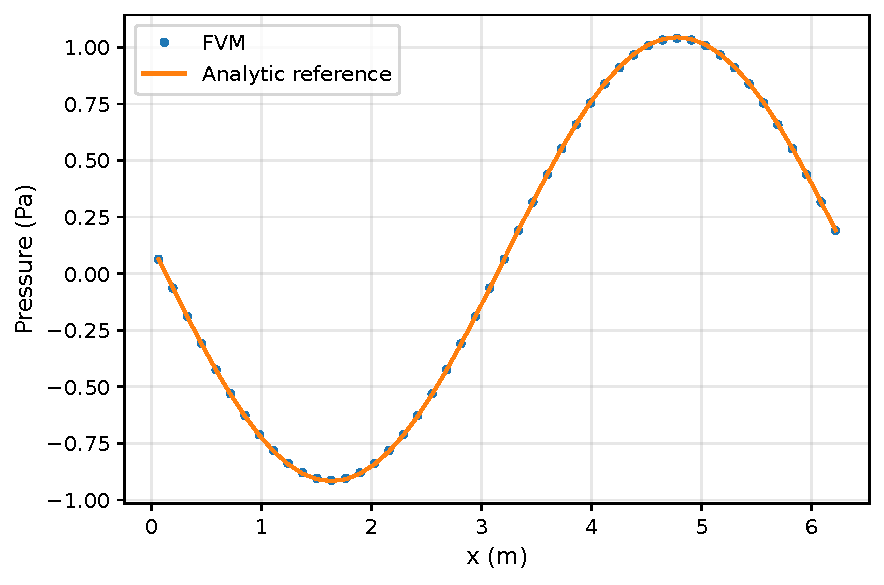
\includegraphics[width=0.48\linewidth]{abc-48/figures/pressure-curve.pdf}
\subsection{advected-shear 32x32x4}
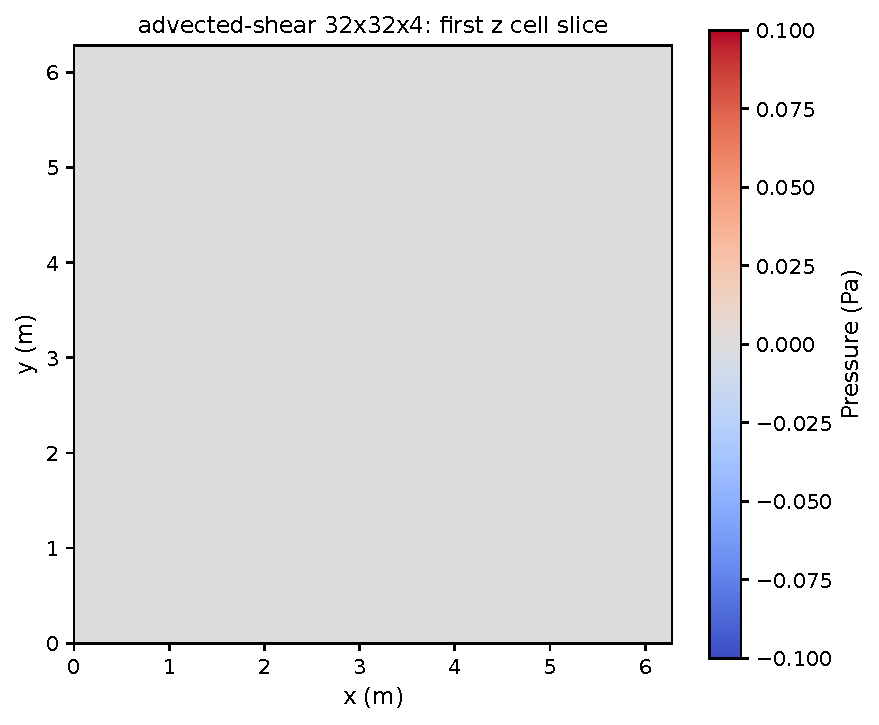
\includegraphics[width=0.48\linewidth]{shear-32/figures/pressure.pdf}
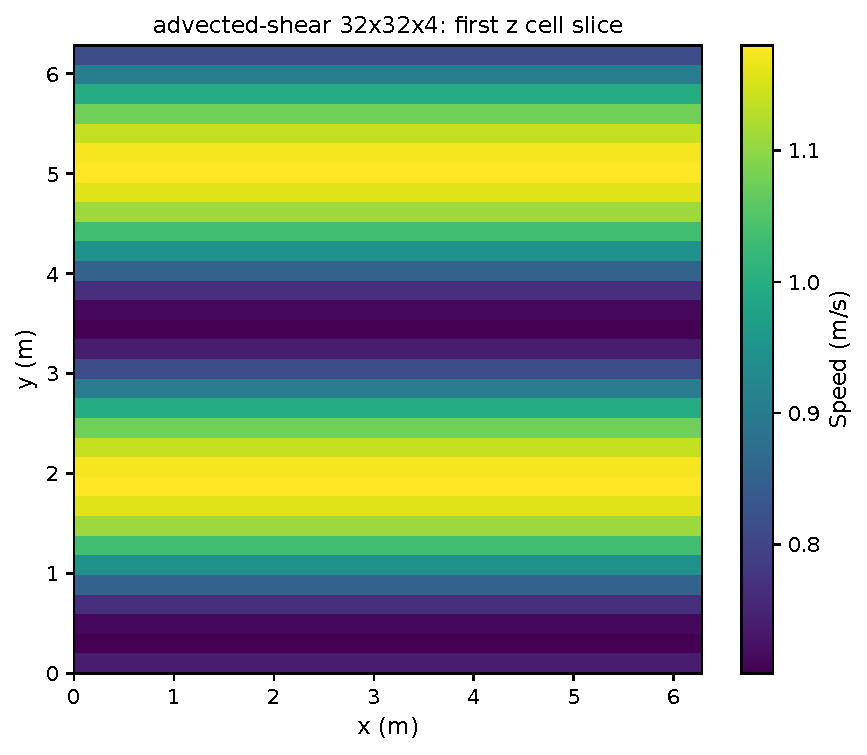
\includegraphics[width=0.48\linewidth]{shear-32/figures/speed.pdf}
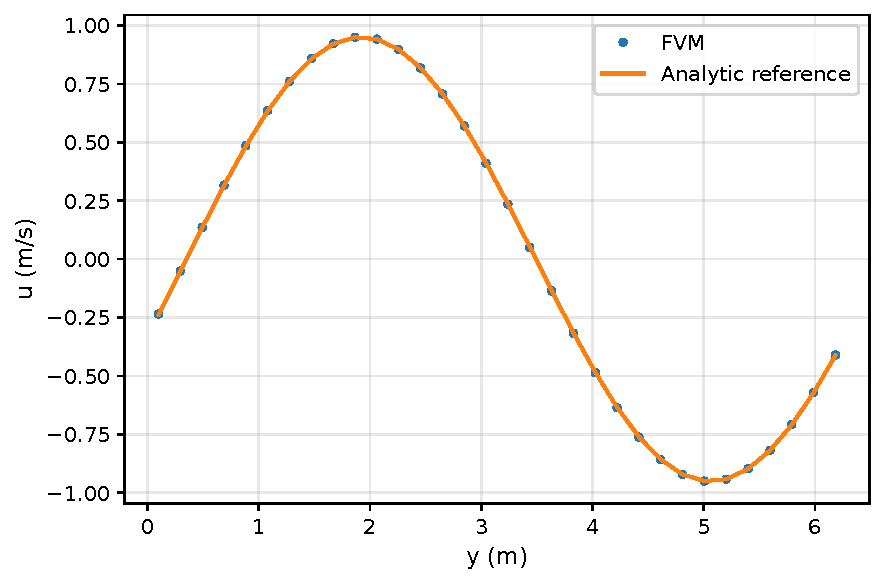
\includegraphics[width=0.48\linewidth]{shear-32/figures/velocity-profile.pdf}
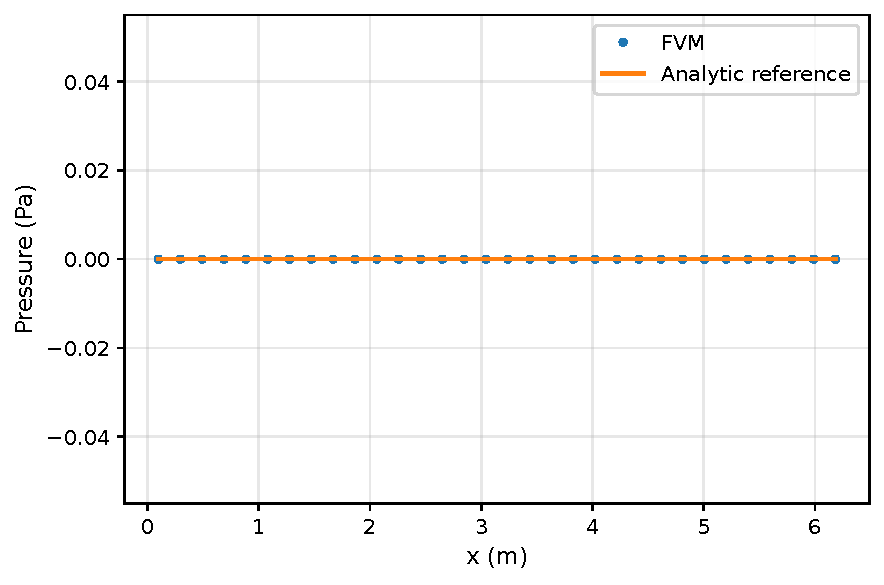
\includegraphics[width=0.48\linewidth]{shear-32/figures/pressure-curve.pdf}
\subsection{advected-shear-lbm 32x32}
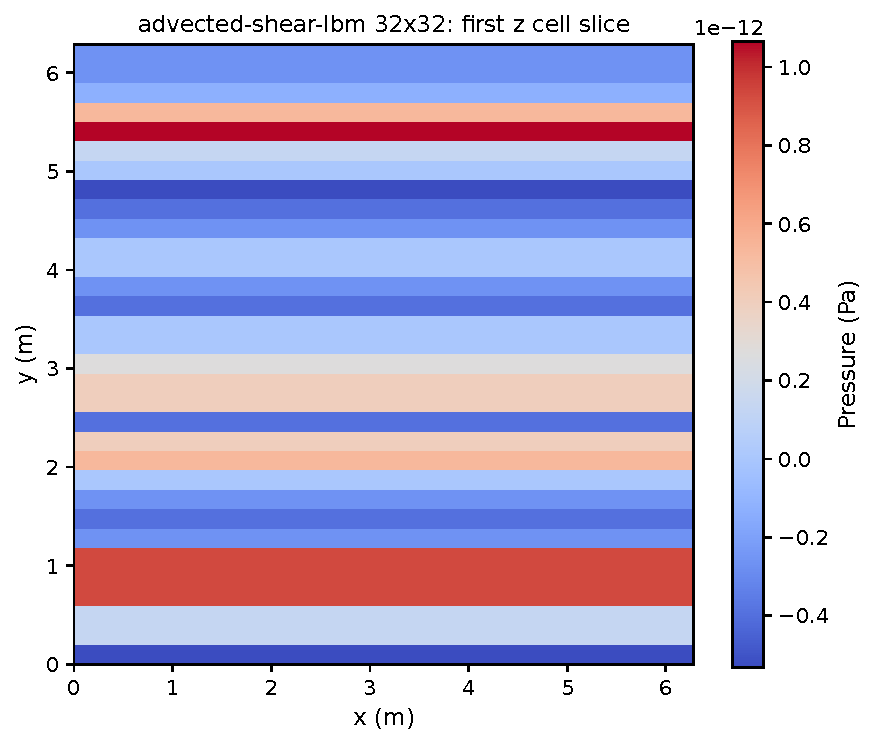
\includegraphics[width=0.48\linewidth]{lbm-shear-32/figures/pressure.pdf}
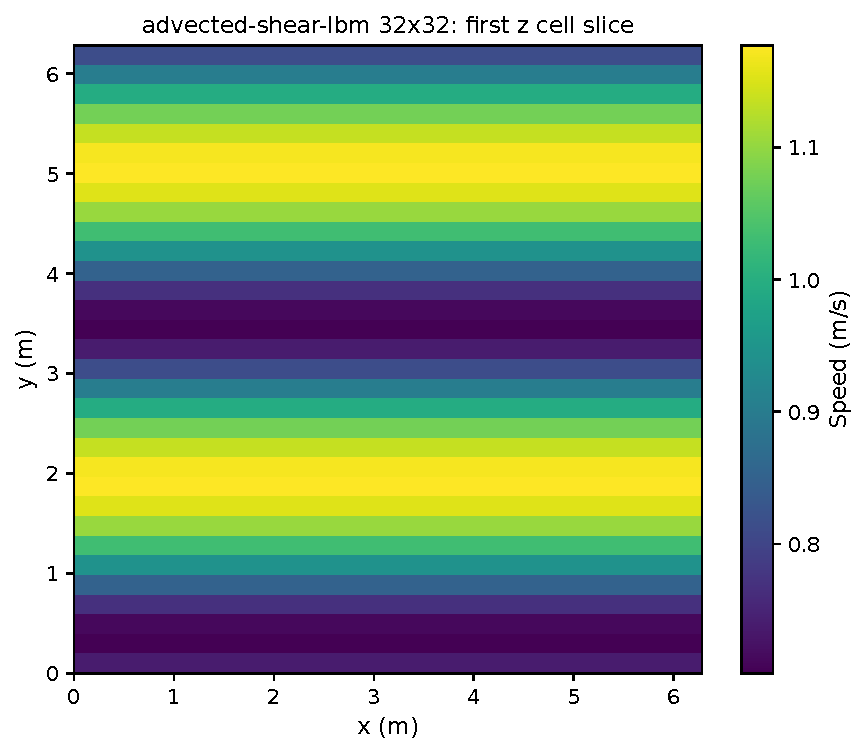
\includegraphics[width=0.48\linewidth]{lbm-shear-32/figures/speed.pdf}
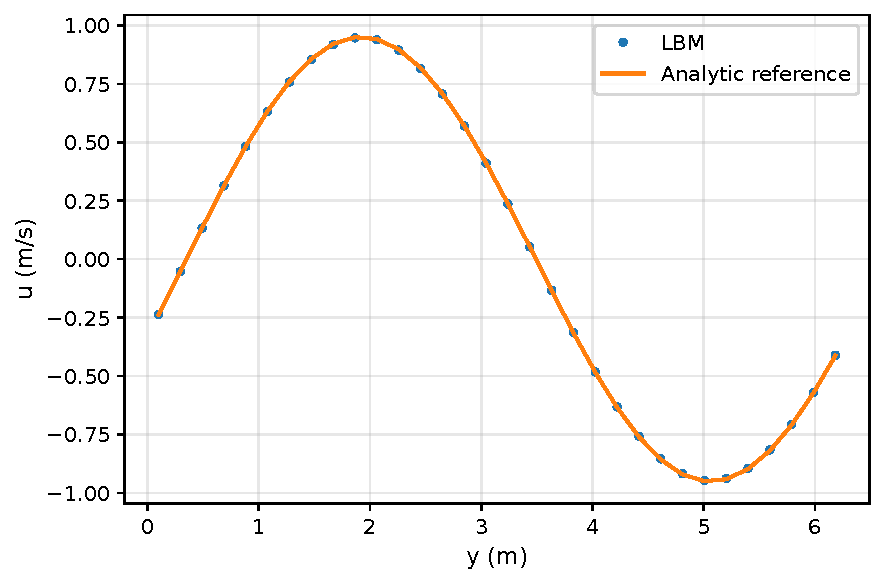
\includegraphics[width=0.48\linewidth]{lbm-shear-32/figures/velocity-profile.pdf}
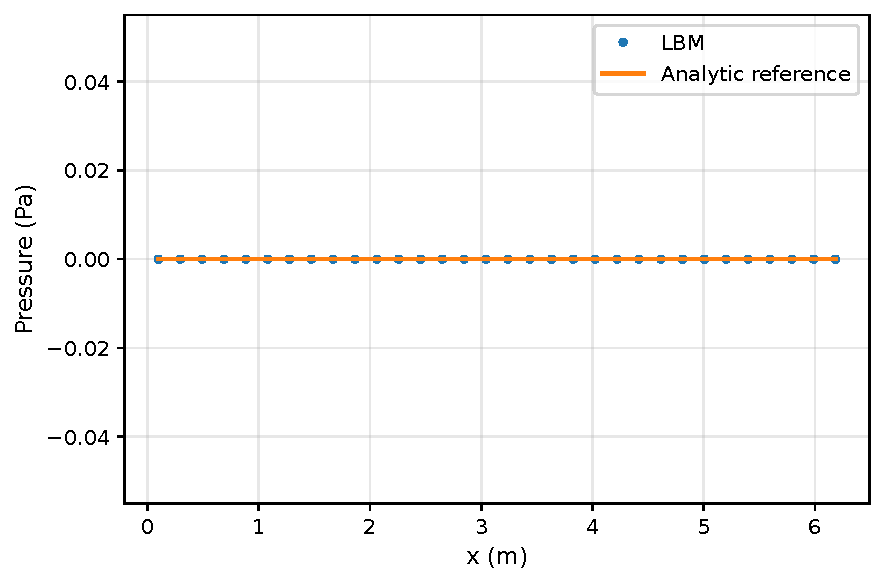
\includegraphics[width=0.48\linewidth]{lbm-shear-32/figures/pressure-curve.pdf}
\end{document}
